\documentclass[border=1cm]{standalone}

\usepackage{tikz}
\usetikzlibrary{3d, calc}

\begin{document}
    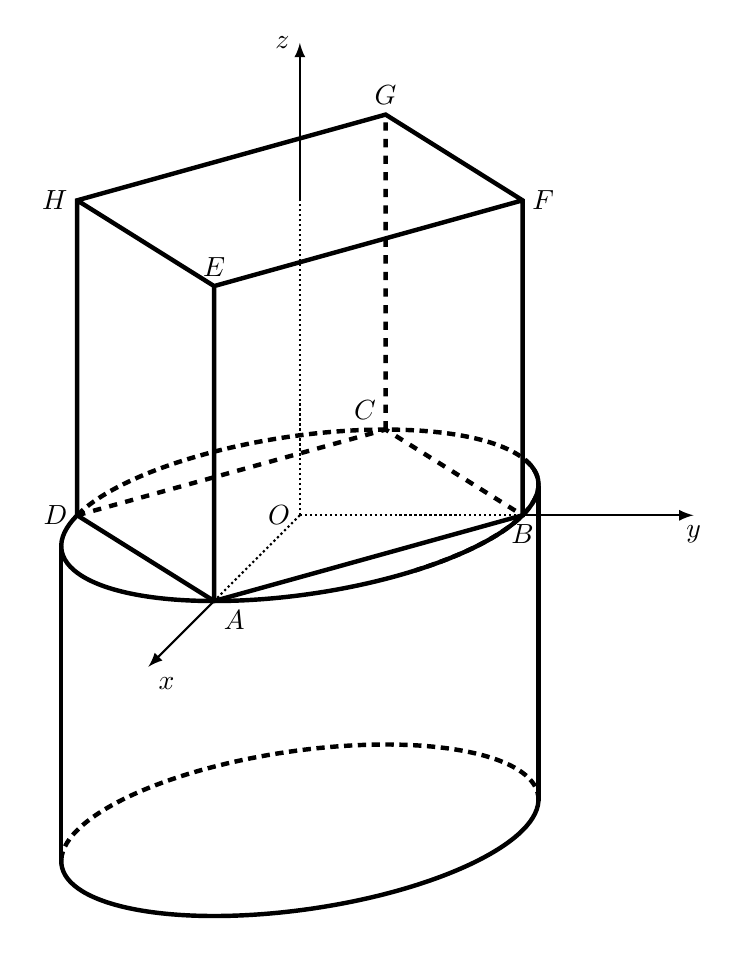
\begin{tikzpicture}
        \coordinate[label=left:$O$] (O) at (0,0,0);
        \coordinate[label=below right:$A$] (A) at (0,0,{2*sqrt(2)});
        \coordinate[label=below:$B$] (B) at ({2*sqrt(2)},0);
        \coordinate[label=above left:$C$] (C) at (0,0,{-2*sqrt(2)});
        \coordinate[label=left:$D$] (D) at ($(A) + (C) - (B)$);
        \coordinate (Z) at (90:4);
        \coordinate[label=above:$E$] (E) at ($(A) + (Z)$);
        \coordinate[label=right:$F$] (F) at ($(B) + (Z)$);
        \coordinate[label=above:$G$] (G) at ($(C) + (Z)$);
        \coordinate[label=left:$H$] (H) at ($(D) + (Z)$);
        \draw[ultra thick](D)--(A)--(B)--(F)--(G)--(H)--cycle (H)--(E)--(F) (E)--(A);
        \draw[ultra thick, dashed](D)--(C)--(B) (C)--(G);

        \begin{scope}[canvas is xz plane at y=0]
            \draw[ultra thick] (B) arc [start angle=0, end angle = 180, radius={2*sqrt(2)}];
            \draw[ultra thick] (B) arc [start angle=0, end angle = -40, radius={2*sqrt(2)}];
            \draw[ultra thick, densely dashed] (D) arc [start angle=-180, end angle = 40, radius={2*sqrt(2)}];
        \end{scope}

        \begin{scope}[rotate around y=20]
            \begin{scope}[canvas is xz plane at y=-4]
                \draw[ultra thick] ({2*sqrt(2)},0) arc [start angle=0, end angle = 180, radius={2*sqrt(2)}];
                \draw[ultra thick, densely dashed] ({-2*sqrt(2)},0) arc [start angle=-180, end angle = 0, radius={2*sqrt(2)}];
            \end{scope}

            \draw[ultra thick] ({2*sqrt(2)},0)--({2*sqrt(2)},-4);
            \draw[ultra thick] ({-2*sqrt(2)},0)--({-2*sqrt(2)},-4);
        \end{scope}

        \draw[thick, densely dotted](0,0)--(B);
        \draw[->,>=latex,thick](B)--(5,0)node[below]{$y$};
        \draw[thick, densely dotted](0,0)--(0,4);
        \draw[->,>=latex,thick](0,4)--(0,6)node[left]{$z$};
        \draw[thick, densely dotted](0,0)--(A);
        \draw[->,>=latex,thick](A)--(0,0,5)node[below right]{$x$};
    \end{tikzpicture}
\end{document}